% Document Class %
\documentclass[11pt, a4paper]{article}

\usepackage[ruled,vlined,linesnumbered]{algorithm2e}
\usepackage{algpseudocode}
\usepackage{amsmath}
\usepackage{amssymb}
\usepackage{bm}
\usepackage{bbding}
\usepackage{caption}
\usepackage{color}
\usepackage{enumitem}
\usepackage{epsfig}
\usepackage{ifpdf}
\usepackage{subfigure}
\usepackage{tikz}
\usepackage{verbatim}
\usepackage{pgfplots}
\usepackage{float}

\usetikzlibrary{arrows,calc,shapes,snakes,automata,backgrounds,fit,petri}
\usetikzlibrary{bayesnet}

\ifpdf
  \DeclareGraphicsRule{*}{mps}{*}{}
\fi

\allowdisplaybreaks

\setlength{\oddsidemargin}{4mm}
\setlength{\evensidemargin}{\oddsidemargin}
\setlength{\textwidth}{160mm}
\setlength{\topmargin}{-5.4mm}
\setlength{\headheight}{5mm}
\setlength{\headsep}{5mm}
\setlength{\footskip}{10mm}
\setlength{\textheight}{230mm}

\def\figures{0}

\newcommand{\norm}[1]{\ensuremath{\left\| #1 \right\|}}
\newcommand{\dataset}{\mathcal{D}}

% A pointer for comments
\def\pointer{\HandRight $\phantom{0}$}

% Math operators
\DeclareMathOperator*{\argmax}{arg\,max}
\def\argmin{\operatornamewithlimits{arg\,min}}
\def\const{\mathop{\rm const}}
\def\cov{\mathop{\rm cov}}
\def\tr{\mathop{\sf tr}}
\def\trace{\mathop{\sf trace}}
\def\var{\mathop{\sf var}}

% Users and items. I think "item" is already a keyword.
\def\usr{\mathop{\rm user}}
\def\itm{\mathop{\rm item}}

% Double bold
\def\Ebb{\mathbb{E}}
\def\Ibb{\mathbb{I}}
\def\Rbb{\mathbb{R}}
\def\Xbb{\mathbb{X}}

% Bold Greek
\def\balpha{\bm{\alpha}}
\def\bbeta{\bm{\beta}}
\def\bmeta{\bm{\eta}}
\def\bgamma{\bm{\gamma}}
\def\bGamma{\mathbf{\Gamma}}
\def\blambda{\bm{\lambda}}
\def\bLambda{\mathbf{\Lambda}}
\def\bmu{\bm{\mu}}
\def\bnu{\bm{\nu}}
\def\bOmega{\mathbf{\Omega}}
\def\bpi{\bm{\pi}}
\def\bPi{\mathbf{\Pi}}
\def\bSigma{\mathbf{\Sigma}}
\def\btau{\bm{\tau}}
\def\btheta{\bm{\theta}}
\def\bTheta{\mathbf{\Theta}}
\def\bxi{\bm{\xi}}
\def\bzeta{\bm{\zeta}}

% Normal bold
\def\0{\mathbf{0}}
\def\a{\mathbf{a}}
\def\b{\mathbf{b}}
\def\c{\mathbf{c}}
\def\d{\mathbf{d}}
\def\e{\mathbf{e}}
\def\f{\mathbf{f}}
\def\k{\mathbf{k}}
\def\m{\mathbf{m}}
\def\r{\mathbf{r}}
\def\s{\mathbf{s}}
\def\u{\mathbf{u}}
\def\v{\mathbf{v}}
\def\x{\mathbf{x}}
\def\y{\mathbf{y}}
\def\z{\mathbf{z}}
\def\A{\mathbf{A}}
\def\B{\mathbf{B}}
\def\C{\mathbf{C}}
\def\D{\mathbf{D}}
\def\E{\mathbf{E}}
\def\F{\mathbf{F}}
\def\G{\mathbf{G}}
\def\H{\mathbf{H}}
\def\I{\mathbf{I}}
\def\J{\mathbf{J}}
\def\K{\mathbf{K}}
\def\L{\mathbf{L}}
\def\P{\mathbf{P}}
\def\R{\mathbf{R}}
\def\S{\mathbf{S}}
\def\U{\mathbf{U}}
\def\V{\mathbf{V}}
\def\W{\mathbf{W}}
\def\X{\mathbf{X}}
\def\Y{\mathbf{Y}}
\def\Z{\mathbf{Z}}

% Brackets
\def\<{ \left\langle }
\def\>{ \right\rangle }

% Caligraphic
\def\Bcal{\mathcal{B}}
\def\Dcal{\mathcal{D}}
\def\Ecal{\mathcal{E}}
\def\Fcal{\mathcal{F}}
\def\Gcal{\mathcal{G}}
\def\Hcal{\mathcal{H}}
\def\Ical{\mathcal{I}}
\def\Lcal{\mathcal{L}}
\def\Mcal{\mathcal{M}}
\def\Ncal{\mathcal{N}}
\def\Ocal{\mathcal{O}}
\def\Rcal{\mathcal{R}}
\def\Scal{\mathcal{S}}
\def\Tcal{\mathcal{T}}
\def\Zcal{\mathcal{Z}}

% General
\def\erm{\mathrm{e}}
\def\wo{\backslash}
\def\defined{\stackrel{\text{\tiny def}}{=}}
\newcommand{\bigE}[1]{{ \big\langle {#1} \big\rangle }}
\newcommand{\BigE}[1]{{ \Big\langle {#1} \Big\rangle }}
\newcommand{\BiggE}[1]{{ \Bigg\langle {#1} \Bigg\rangle }}

\definecolor{Blue}{rgb}{0.0,0.0,1.0}
\newcommand{\bluetext}[1]{{\color{Blue}{#1}}}

\definecolor{White}{rgb}{1.0,1.0,1.0}
\newcommand{\whitetext}[1]{{\color{White}{#1}}}


\begin{document}

\title{Radio Paper Model and Algorithm}

\maketitle

\section{ Graphical Model}

In the radio paper we have bayesian model best visualized as the following graphical model:

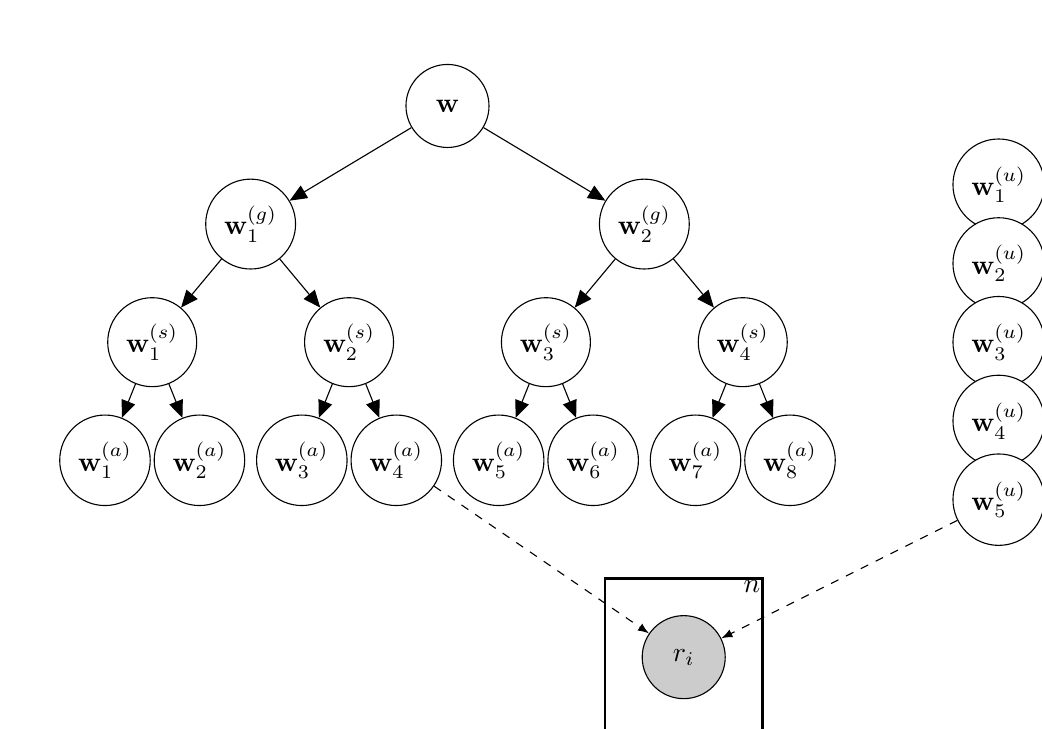
\begin{tikzpicture}[darkstyle/.style={circle,draw,fill=white!40,minimum size=30}]
\tikzstyle{obsnode}=[circle,draw,fill=gray!40,minimum size=30]
\tikzstyle{plate}=[draw,thick,minimum width=2cm,minimum height=2cm]
\tikzstyle{line}=[draw]
\tikzstyle{arrow}=[draw, -latex,dashed]
  \tikzstyle{level 1}=[sibling distance=50mm]
   \tikzstyle{level 2}=[sibling distance=25mm]
    \tikzstyle{level 3}=[sibling distance=12mm]
    \tikzstyle{level 4}=[sibling distance=6mm]
    \tikzstyle{level 5}=[sibling distance=4mm,level distance=10mm]
     \node[darkstyle]{\textbf{w}} child[->] foreach \g in {1,2}
                                {node[darkstyle] {$\textbf{w}^{(g)}_{\g}$} child[->] foreach \t [evaluate={\s=int(\g*2+\t-1);}] in {0,1}
                                         { node[darkstyle] {$\textbf{w}^{(s)}_{\s}$} child[->] foreach \q [evaluate={\a=int(\s*2+\q-1);}] in {0,1}
                                         {node[darkstyle] (a\a) {$\textbf{w}^{(a)}_{\a}$} }}};
     \foreach \u in {1,...,5}
            {\pgfmathtruncatemacro{\label}{\u}
        \node[darkstyle] (u\u) at (7,0-\u){$\textbf{w}^{(u)}_\label$};}

        \node[plate] (p) at (3,-7){} ;
        \node[obsnode](r) at (3,-7){$r_{i}$};
        \node[anchor=north east,inner sep=1pt] at (p.north east){$n$};
        \path[arrow]  (u5) -- (r){};
        \path[arrow]  (a4) -- (r){};

        \end{tikzpicture}

\section{Notation}
We define the following notation:\begin{itemize}
                                   \item $r_i\in \{0,1\}$ is the rating of example $i$
                                   \item $\textbf{x}_i\in \mathbb{R}^D$ is the set of features for example $i$
                                   \item $\textbf{w} \in \mathbb{R}^D$ is the global weight vector
                                   \item $\textbf{w}^{(g)}_k \in \mathbb{R}^D$ is the genere weight vector for genre $k$
                                   \item $\textbf{w}^{(s)}_k \in \mathbb{R}^D$ is the subgenere weight vector for subgenre $k$
                                   \item $\textbf{w}^{(a)}_k \in \mathbb{R}^D$ is the artist weight vector for artist $k$
                                   \item $\textbf{w}^{(u)}_p \in \mathbb{R}^D$ is the user weight vector for user $p$
                                   \item $\mathcal{G}(i)$ denotes the genere index of example $i$
                                   \item $\mathcal{S}(i)$ denotes the subgenere index of example $i$
                                   \item $\mathcal{A}(i)$ denotes the artist index of example $i$
                                   \item $\mathcal{U}(i)$ denotes the user index of example $i$
                                   \item $N$ denotes the total number of training examples
                                   \item $K_g$ denotes the total number of generes
                                   \item $K_s$ denotes the total number of subgeneres
                                   \item $K_a$ denotes the total number of artists
                                   \item $K_u$ denotes the total number of users
                                   \item  \texttt{parent}(\textbf{y}) is a function mapping from node \textbf{y} to its parent in the hierarchy
                                   \item  \texttt{children}(\textbf{y}) is a function mapping from node \textbf{y} to the set of its children in the hierarchy

                                 \end{itemize}

\section{Likelihood}

We consider the following likelihood:
$$L\left(\mathcal{W}\right)=\prod_{i=1}^N P\left(r_i \mid \textbf{x}_i , \textbf{w}^{(a)}_{\mathcal{A}(i)}, \textbf{w}^{(u)}_{\mathcal{U}(i)} \right)$$

\noindent Using indicator functions it can be written more precisely as:
$$L\left(\mathcal{W}\right)=\prod_{i=1}^N \prod_{k=1}^{K_a}\prod_{p=1}^{K_u}P\left(r_i \mid \textbf{x}_i , \textbf{w}^{(a)}_{k}, \textbf{w}^{(u)}_{p} \right)^{\mathbb{I}\left[\mathcal{A}(i)=k,\mathcal{U}(i)=p\right]}$$

\noindent Since we have a binary decision problem our sampling distribution, $P\left(r_i \mid \textbf{x}_i , \textbf{w}^{(a)}_{k}, \textbf{w}^{(u)}_{p} \right)$, is bernoulli with parameter $\sigma\left(\left(\textbf{w}^{(u)}_{p} +\textbf{w}^{(a)}_{k}\right)^\top \textbf{x}_i\right)=\frac{1}{1+\exp\left[-\left(\textbf{w}^{(u)}_{p} +\textbf{w}^{(a)}_{k}\right)^\top \textbf{x}_i\right]}$ thus:

$$L\left(\mathcal{W}\right)=\prod_{i=1}^N \prod_{k=1}^{K_a}\prod_{p=1}^{K_u} \left(\left(\sigma\left(\left(\textbf{w}^{(u)}_{p} +\textbf{w}^{(a)}_{k}\right)^\top \textbf{x}_i\right)\right)^{r_i}+ \left(1-\sigma\left(\left(\textbf{w}^{(u)}_{p} +\textbf{w}^{(a)}_{k}\right)^\top \textbf{x}_i\right)\right)^{\left(1-r_i\right)}\right)^{\mathbb{I}\left[\mathcal{A}(i)=k,\mathcal{U}(i)=p\right]}$$

\subsection{Lower Bound on the log likelihood}

In order to facilitate the variational (mean field) approximation we will bound the log-likelihood from below using a function that is quadratic in our parameters $\textbf{w}^{(a)}$ and $\textbf{w}^{(u)}$. The tradeoff is the addition of an additional variational parameter $\xi_i$ for every training example index $i$. We begin by writing the log-likelihood:

\begin{align*}\ell(\mathcal{W})&=\log\left[L\left(\mathcal{W}\right)\right]\\
&=\sum_{i=1}^N \sum_{k=1}^{K_a}\sum_{p=1}^{K_u} \bigg[\mathbb{I}\left[\mathcal{A}(i)=k,\mathcal{U}(i)=p\right]\cdot\\
 &\qquad{}\qquad{}\qquad{}\left.\left(r_i\log\left(\sigma\left(\left(\textbf{w}^{(u)}_{p} +\textbf{w}^{(a)}_{k}\right)^\top \textbf{x}_i\right)\right)+ {\left(1-r_i\right)}\log\left(1-\sigma\left(\left(\textbf{w}^{(u)}_{p} +\textbf{w}^{(a)}_{k}\right)^\top \textbf{x}_i\right)\right)\right)\right]
 \end{align*}

\noindent Next we consider the following variational bound on the logistic sigmoid : $$\sigma(x)\geq \sigma(\xi)\exp\left\{\frac{x-\xi}{2}-\lambda(\xi)\left(x^2-\xi^2\right)\right\}=f(x,\xi)$$

\noindent where $\xi$ is the new variational parameter and $\lambda(\xi)=\frac{1}{2\xi}\left[\sigma(\xi)-\frac{1}{2}\right]$.

\noindent For a given value of $x$, the value of $\xi$ that maximizes $f(x,\xi)$,thus giving the tightest lower bound on $\sigma(x)$ has a closed form solution:

$$\left(\xi^*\right)^2=\left(\argmax_\xi f(x,\xi)\right)^2= x^2$$

\noindent Due to the monotonicity of logarithms $\xi^*$ is also the maximizer of $\log\left( f(x,\xi)\right)$ and $\log\left(\sigma(x)\right)\geq \log\left( f(x,\xi)\right)= \log\left(\sigma(\xi)\right)+\frac{x-\xi}{2}-\lambda(\xi)\left(x^2-\xi^2\right)$. We also make the following observation:
$$\sigma(x)^r\left(1-\sigma(x)\right)^{\left(1-r\right)}=e^{xr}\sigma(-x)\Leftrightarrow  r\log\left(\sigma(x)\right)+\left(1-r\right)\log\left(1-\sigma(x)\right)=xr+\log\left(\sigma(-x)\right)$$

\noindent Using all these we can finally write the lower bound on the loglikelihood:
\begin{align*}
\ell(\mathcal{W})&=\\
&=\sum_{i=1}^N \sum_{k=1}^{K_a}\sum_{p=1}^{K_u} \bigg[\mathbb{I}\left[\mathcal{A}(i)=k,\mathcal{U}(i)=p\right]\cdot\\
&\qquad{}\qquad{}\qquad{}\left(\left(r_i\cdot\left(\textbf{w}^{(u)}_{p} +\textbf{w}^{(a)}_{k}\right)^\top \textbf{x}_i\right) + \log\left(\sigma\left(-\left(\textbf{w}^{(u)}_{p} +\textbf{w}^{(a)}_{k}\right)^\top \textbf{x}_i\right)\right)\right)\bigg]\\
&\geq\sum_{i=1}^N \sum_{k=1}^{K_a}\sum_{p=1}^{K_u} \Bigg[\mathbb{I}\left[\mathcal{A}(i)=k,\mathcal{U}(i)=p\right]\cdot\bigg[\left(r_i\cdot\left(\textbf{w}^{(u)}_{p} +\textbf{w}^{(a)}_{k}\right)^\top \textbf{x}_i\right)+\\
&\qquad{}\qquad{}\qquad{}\left(\log\left(\sigma(\xi_i)\right)+\frac{\left(-\left(\textbf{w}^{(u)}_{p} +\textbf{w}^{(a)}_{k}\right)^\top \textbf{x}_i\right)-\xi_i}{2}-\lambda(\xi_i)\left(\left(\left(\textbf{w}^{(u)}_{p} +\textbf{w}^{(a)}_{k}\right)^\top \textbf{x}_i\right)^2-\xi_i^2\right)\right)\bigg]\Bigg]\\
&= \ell(\mathcal{W},\left\{\xi_i\right\}_{i=1}^N)\\
\end{align*}

\section{Prior}

We are now ready to define our hierarchical prior. The overall prior takes the following form, utilizing the conditional independence structure of the graph:
\begin{align*}
P(\mathcal{W})=P(\textbf{w}) \times &\prod_{k_1=1}^{K_g}P\left(\textbf{w}^{(g)}_{k_1} \mid \texttt{parent}(\textbf{w}^{(g)}_{k_1})\right)\times\\
&\prod_{k_2=1}^{K_s}P\left(\textbf{w}^{(s)}_{k_2} \mid \texttt{parent}(\textbf{w}^{(s)}_{k_2})\right)\times \prod_{k_3=1}^{K_a}P\left(\textbf{w}^{(a)}_{k_3} \mid \texttt{parent}(\textbf{w}^{(a)}_{k_3})\right)\times\prod_{p=1}^{K_u}P\left(\textbf{w}^{(u)}_{p} \right)\end{align*}

\noindent We define the specific components of the prior below where all members of the same semantic family of variables share a single prior precision parameter.
\paragraph{The global prior:}
$$P(\textbf{w})=\mathcal{N}\left(\textbf{w}; \textbf{0}_D, \alpha^{-1}\cdot \textbf{I}_D \right)$$
\noindent Where $\textbf{0}_D$ is the $D$-dimensional zero vector and $\textbf{I}_D$ is the $D \times D$ Identity matrix.

\paragraph{The genere priors:}
\noindent for $k=1\dots K_g$ we define:
$$P\left(\textbf{w}^{(g)}_{k} \mid \texttt{parent}(\textbf{w}^{(g)}_{k})\right)=\mathcal{N}\left(\textbf{w}^{(g)}_{k}; \textbf{w}, \alpha_g^{-1}\cdot \textbf{I}_D \right)$$

\paragraph{The subgenere priors:}
\noindent for $k=1\dots K_s$ we define:
$$P\left(\textbf{w}^{(s)}_{k} \mid \texttt{parent}(\textbf{w}^{(s)}_{k})\right)=\mathcal{N}\left(\textbf{w}^{(s)}_{k}; \textbf{w}^{(g)}_{\texttt{par}}, \alpha_s^{-1}\cdot \textbf{I}_D \right)$$
\noindent where  $\textbf{w}^{(g)}_{\texttt{par}}=\texttt{parent}(\textbf{w}^{(s)}_{k})$ denotes the parent of subgenere node in the genre layer of the hierarchy.

\paragraph{The artist priors:}
\noindent for $k=1\dots K_a$ we define:
$$P\left(\textbf{w}^{(a)}_{k} \mid \texttt{parent}(\textbf{w}^{(a)}_{k})\right)=\mathcal{N}\left(\textbf{w}^{(a)}_{k}; \textbf{w}^{(s)}_{\texttt{par}}, \alpha_a^{-1}\cdot \textbf{I}_D \right)$$

\noindent where  $\textbf{w}^{(s)}_{\texttt{par}}=\texttt{parent}(\textbf{w}^{(a)}_{k})$ denotes the parent of artist node in the subgenre layer of the hierarchy.

\paragraph{The user priors:}
\noindent for $p=1\dots K_u$ we define:
$$P\left(\textbf{w}^{(u)}_{p}\right)=\mathcal{N}\left(\textbf{w}^{(u)}_{p}; \textbf{0}_D, \alpha_u^{-1}\cdot \textbf{I}_D \right)$$

\section{The Log Joint Distribution}

In this section we will make explicit the full form of the log joint distribution over all data and variables. This expression is  will serve us when constructing the variational approximation. The log of the full joint distribution is given by the following:

\begin{multline*}
\log\left(P\left(\mathcal{W},\left\{x_i\right\}_{i=1}^N,\left\{r_i\right\}_{i=1}^N \mid \left\{\xi_i\right\}_{i=1}^N\right)\right)=\ell(\mathcal{W},\left\{\xi_i\right\}_{i=1}^N)+\log\left(P(\mathcal{W})\right)\\
=\ell(\mathcal{W},\left\{\xi_i\right\}_{i=1}^N)+\log\left(P(\textbf{w})\right) + \sum_{k_1=1}^{K_g}\log\left(P\left(\textbf{w}^{(g)}_{k_1} \mid \texttt{parent}(\textbf{w}^{(g)}_{k_1})\right)\right)+\\
\sum_{k_2=1}^{K_s}\log\left(P\left(\textbf{w}^{(s)}_{k_2} \mid \texttt{parent}(\textbf{w}^{(s)}_{k_2})\right)\right)+ \sum_{k_3=1}^{K_a}\log\left(P\left(\textbf{w}^{(a)}_{k_3} \mid \texttt{parent}(\textbf{w}^{(a)}_{k_3})\right)\right)+\sum_{p=1}^{K_u}\log\left(P\left(\textbf{w}^{(u)}_{p} \right)\right)
\end{multline*}

\noindent Now let us consider the explicit form of the components of this expression:
\begin{itemize}
  \item $\ell(\mathcal{W},\left\{\xi_i\right\}_{i=1}^N)$ is given in explicit form in section 3.1
  \item $\log\left(P(\textbf{w})\right)=-\frac{\alpha}{2}\left(\textbf{w}^\top\textbf{w}\right)$
  \item $\log\left(P\left(\textbf{w}^{(g)}_{k_1} \mid \texttt{parent}(\textbf{w}^{(g)}_{k_1})\right)\right)=-\frac{\alpha_g}{2}\left(\left(\textbf{w}^{(g)}_{k_1}-\textbf{w}\right)^\top\left(\textbf{w}^{(g)}_{k_1}-\textbf{w}\right)\right)$
  \item $\log\left(P\left(\textbf{w}^{(s)}_{k_2} \mid \texttt{parent}(\textbf{w}^{(s)}_{k_2})\right)\right)=-\frac{\alpha_s}{2}\left(\left(\textbf{w}^{(s)}_{k_2}-\textbf{w}^{(g)}_{\texttt{par}}\right)^\top\left(\textbf{w}^{(s)}_{k_2}-\textbf{w}^{(g)}_{\texttt{par}}\right)\right)$\\
      where  $\textbf{w}^{(g)}_{\texttt{par}}=\texttt{parent}(\textbf{w}^{(s)}_{k_2})$
   \item $\log\left(P\left(\textbf{w}^{(a)}_{k_3} \mid \texttt{parent}(\textbf{w}^{(a)}_{k_3})\right)\right)=-\frac{\alpha_a}{2}\left(\left(\textbf{w}^{(a)}_{k_3}-\textbf{w}^{(s)}_{\texttt{par}}\right)^\top\left(\textbf{w}^{(a)}_{k_3}-\textbf{w}^{(s)}_{\texttt{par}}\right)\right)$\\
      where  $\textbf{w}^{(a)}_{\texttt{par}}=\texttt{parent}(\textbf{w}^{(a)}_{k_3})$
   \item $\log\left(P\left(\textbf{w}^{(u)}_{p} \right)\right)=-\frac{\alpha_u}{2}\left({\textbf{w}^{(u)}_{p}}^\top\textbf{w}^{(u)}_{p} \right)$
\end{itemize}

\section{Variational Approximation and Learning Algorithm}

\noindent Our approach to learning is to combine mean field approximation for the hierarchy with EM for maximizing the variational lower bound. Thus we use the following approximation to the posterior which fully factors across all variables in the hierarchy:

\begin{align*}
q(\mathcal{W})
=q(\textbf{w}) \times &\prod_{k_1=1}^{K_g}q\left(\textbf{w}^{(g)}_{k_1}\right)\times\\
&\prod_{k_2=1}^{K_s}q\left(\textbf{w}^{(s)}_{k_2} \right)\times \prod_{k_3=1}^{K_a}q\left(\textbf{w}^{(a)}_{k_3}\right)\times\prod_{p=1}^{K_u}q\left(\textbf{w}^{(u)}_{p} \right)
\end{align*}


\subsection{Algorithm 1: VB +EM}
\noindent This approximation defines the following lower bound on the log evidence:
$$F\left(q(\mathcal{W}),\left\{\xi\right\}_{i=1}^N\right)=\int q(\mathcal{W})\log\left(\frac{\log\left(P\left(\mathcal{W},\left\{x_i\right\}_{i=1}^N,\left\{r_i\right\}_{i=1}^N \mid \left\{\xi_i\right\}_{i=1}^N\right)\right)}{q(\mathcal{W})} \right) d\mathcal{W}$$



\noindent Our algorithm  iterates over the following two steps until convergence of $F\left(q(\mathcal{W}),\left\{\xi\right\}_{i=1}^N\right)$:
\begin{enumerate}
                                              \item Estimate the variational posterior using ``Variational Bayes" keeping the variational parameters ($\xi$) fixed (Maximize $F\left(q(\mathcal{W}),\left\{\xi\right\}_{i=1}^N\right)$ w.r.t. $q(\mathcal{W})$):
                                              \begin{enumerate}
                                                \item \begin{tabbing}
Repeat \= until convergence of $F\left(q(\mathcal{W}),\left\{\xi\right\}_{i=1}^N\right)$ ($\xi_i$'s are fixed): \\
\>For \=each $w_i$ in the hierarchy and users:\\
\>\>$\log\left(q(w_i)\right)=\mathbb{E}_{j\neq i} \left[\log\left(P\left(\mathcal{W},\left\{x_i\right\}_{i=1}^N,\left\{r_i\right\}_{i=1}^N \mid \left\{\xi_i\right\}_{i=1}^N\right)\right)\right]$\\

\end{tabbing}



                                              \end{enumerate}
                                              \item Perform analytical maximization of the variational parameters (Maximize $F\left(q(\mathcal{W}),\left\{\xi\right\}_{i=1}^N\right)$ w.r.t. $\left\{\xi\right\}_{i=1}^N$)
                                               \begin{enumerate}
                                                \item \begin{tabbing}
For \= $i=1\dots N$:\\
\>$\xi_i=\argmax_{\xi_i}\left(\mathbb{E}_{q(\mathcal{W})} \left[\log\left(P\left(\mathcal{W},\left\{x_i\right\}_{i=1}^N,\left\{r_i\right\}_{i=1}^N \mid \left\{\xi_i\right\}_{i=1}^N\right)\right)\right]\right)$\\
\end{tabbing}
                                            \end{enumerate}
                                              \end{enumerate}

\subsection{Algorithm 2: VB Only}

 In this algorithm we would like to avoid the requirement of keeping around all the $\left\{\xi\right\}_{i=1}^N$ variational parameters. To that end we note that:
 \begin{align*}
 F\left(q(\mathcal{W})\right)&=\int q(\mathcal{W})\log\left(\frac{\log\left(P\left(\mathcal{W},\left\{x_i\right\}_{i=1}^N,\left\{r_i\right\}_{i=1}^N \right)\right)}{q(\mathcal{W})} \right) d\mathcal{W} \\&\geq \int q(\mathcal{W})\log\left(\frac{\log\left(P\left(\mathcal{W},\left\{x_i\right\}_{i=1}^N,\left\{r_i\right\}_{i=1}^N \mid \left\{\xi_i\right\}_{i=1}^N\right)\right)}{q(\mathcal{W})} \right) d\mathcal{W}=F\left(q(\mathcal{W}),\left\{\xi\right\}_{i=1}^N\right)\\\end{align*}

Thus the algorithm now iterates until convergence of $ F\left(q(\mathcal{W})\right)$:
\begin{enumerate}
                                   \item \begin{tabbing}
Repeat \= until convergence of $F\left(q(\mathcal{W})\right)$ : \\
\>For \=each $w_i$ in the hierarchy and users:\\
\>\>$\xi^*_k= \argmax_{\xi_k}\left(\mathbb{E} \left[\log\left(P\left(\mathcal{W},\left\{x_i\right\}_{i=1}^N,\left\{r_i\right\}_{i=1}^N \mid \left\{\xi_i\right\}_{i=1}^N\right)\right)\right]\right)$ \\
\>\>$\log\left(q(w_i)\right)=\mathbb{E}_{j\neq i} \left[\log\left(P\left(\mathcal{W},\left\{x_i\right\}_{i=1}^N,\left\{r_i\right\}_{i=1}^N \mid \left\{\xi^*_k\right\}_{k=1}^N\right)\right)\right]$\\

\end{tabbing}

\end{enumerate}


\section{The update equations}

Deriving the update equations can be done as follows, when considering a particular variable $\textbf{y}$ , write down all the terms in the log joint distribution of Section 5 that contain this variable. Since we have taken great care in choosing our model, these terms should all be quadratic or linear in $\textbf{y}$, and thus the corresponding distribution is a gaussian. Group the quadratic terms, this expression will give your precision matrix. Group the linear terms, this expression will give you the mean (mean times precision actually) of the gaussian.
If we encounter any parameters not in  $\textbf{y}$ , we will assume their expectation is known by our factorization assumption, and plug in this value.
The sole exception to this technique is optimizing for the $\xi$ variational parameters. In this case we simply maximize the log joint distribution (from section 5) with respect to the relevant example.

\paragraph{Update for global parameter}
$$q(\textbf{w})=\mathcal{N}\left(\textbf{w}; \mu, \Sigma \right)$$
$$\Sigma=\left[\left(\alpha+K_g\cdot\alpha_g\right)\cdot  \textbf{I}_D \right]^{-1}$$
$$\mu=\Sigma\cdot\left[\alpha_g\sum_{k=1}^{K_g}\mathbb{E}\left[\textbf{w}^{(g)}_{k}\right] \right]$$

\noindent where $\mathbb{E}\left[\cdot\right]$ denotes expectation

\paragraph{Update for genere parameters}
\noindent for $k=1\dots K_g$ we define:

$$q(\textbf{w}^{(g)}_{k})=\mathcal{N}\left(\textbf{w}^{(g)}_{k}; \mu^{(g)}_k, \Sigma^{(g)}_k \right)$$
$$\Sigma^{(g)}_k =\left[\left(\alpha_g+|\mathcal{C}_k|\cdot\alpha_s\right)\cdot  \textbf{I}_D \right]^{-1}$$
$$\mu^{(g)}_k=\Sigma^{(g)}_k \cdot\left[\alpha_g\cdot \mathbb{E}\left[\textbf{w}\right]+\alpha_s\sum_{\textbf{w}^{(s)}_{i}\in \mathcal{C}_k}\mathbb{E}\left[\textbf{w}^{(s)}_{i}\right] \right]$$

\noindent where $\mathcal{C}_k=\texttt{children}\left(\textbf{w}^{(g)}_{k}\right)$ denotes the set of child nodes of node $\textbf{w}^{(g)}_{k}$ in the subgenere layer of the hierarchy

\paragraph{Update for subgenere parameters}
\noindent for $k=1\dots K_s$ we define:

$$q(\textbf{w}^{(s)}_{k})=\mathcal{N}\left(\textbf{w}^{(s)}_{k}; \mu^{(s)}_k, \Sigma^{(s)}_k \right)$$
$$\Sigma^{(s)}_k =\left[\left(\alpha_s+|\mathcal{C}_k|\cdot\alpha_a\right)\cdot  \textbf{I}_D \right]^{-1}$$
$$\mu^{(s)}_k=\Sigma^{(s)}_k \cdot\left[\alpha_s\cdot \mathbb{E}\left[\textbf{w}^{(g)}_{\texttt{par}}\right]+\alpha_a\sum_{\textbf{w}^{(a)}_{i}\in \mathcal{C}_k}\mathbb{E}\left[\textbf{w}^{(a)}_{i}\right] \right]$$

\noindent where $\mathcal{C}_k=\texttt{children}\left(\textbf{w}^{(s)}_{k}\right)$ denotes the set of child nodes of node $\textbf{w}^{(s)}_{k}$ in the artist layer of the hierarchy and $\textbf{w}^{(g)}_{\texttt{par}}=\texttt{parent}\left(\textbf{w}^{(s)}_{k}\right)$ is the parent node of node $\textbf{w}^{(s)}_{k}$ in the genere layer of the hierarchy.

\paragraph{Update for artist parameters}
\noindent for $k=1\dots K_a$ we define:
$$q(\textbf{w}^{(a)}_{k})=\mathcal{N}\left(\textbf{w}^{(a)}_{k}; \mu^{(a)}_k, \Sigma^{(a)}_k \right)$$
$$\Sigma^{(a)}_k =\left[\left(\alpha_a \cdot \textbf{I}_D+\sum_{i=1}^N \mathbb{I}\left[\mathcal{A}(i)=k\right]2\lambda(\xi_i)\textbf{x}_i\textbf{x}_i^\top  \right)\right]^{-1}$$
$$\mu^{(a)}_k=\Sigma^{(a)}_k \cdot\left[\alpha_a\cdot \mathbb{E}\left[\textbf{w}^{(s)}_{\texttt{par}}\right]+\sum_{i=1}^N \sum_{p=1}^{K_u} \mathbb{I}\left[\mathcal{A}(i)=k,\mathcal{U}(i)=p\right] \cdot \left( \textbf{x}_i\left(r_i-\frac{1}{2} - 2\lambda(\xi_i) \textbf{x}_i^\top\mathbb{E}\left[\textbf{w}^{(u)}_{p}\right]\right)\right)\right]$$
%\mathbb{I}\left[\mathcal{A}(i)=k,\mathcal{U}(i)=p\right]

\noindent where $\textbf{w}^{(s)}_{\texttt{par}}=\texttt{parent}\left(\textbf{w}^{(a)}_{k}\right)$ is the parent node of node $\textbf{w}^{(a)}_{k}$ in the subgenere layer of the hierarchy.

\paragraph{Update for user parameters}
\noindent for $p=1\dots K_u$ we define:
$$q(\textbf{w}^{(u)}_{p})=\mathcal{N}\left(\textbf{w}^{(u)}_{p}; \mu^{(u)}_p, \Sigma^{(u)}_p \right)$$
$$\Sigma^{(u)}_p =\left[\alpha_u \cdot \textbf{I}_D +\left(\sum_{i=1}^N \mathbb{I}\left[\mathcal{U}(i)=p\right]2\lambda(\xi_i)\textbf{x}_i\textbf{x}_i^\top  \right)\right]^{-1}$$
$$\mu^{(u)}_p=\Sigma^{(u)}_p \cdot\left[\sum_{i=1}^N \sum_{k=1}^{K_a} \mathbb{I}\left[\mathcal{A}(i)=k,\mathcal{U}(i)=p\right] \cdot \left( \textbf{x}_i\left(r_i-\frac{1}{2} - 2\lambda(\xi_i) \textbf{x}_i^\top\mathbb{E}\left[\textbf{w}^{(a)}_{k}\right]\right)\right)\right]$$

\paragraph{Update for variational parameters}
\noindent for $i=1\dots N$ we define:
$$k=\mathcal{A}(i)$$
$$p=\mathcal{U}(i)$$
$\mathbb{E}_{q(\mathcal{W})} \left[\log\left(P\left(\mathcal{W},\left\{x_i\right\}_{i=1}^N,\left\{r_i\right\}_{i=1}^N \mid \left\{\xi_i\right\}_{i=1}^N\right)\right)\right]$ is maximized for $\xi_i^2=\mathbb{E}\left[\left(\left(\textbf{w}^{(a)}_{k}+\textbf{w}^{(u)}_{p}\right)^\top\textbf{x}_i\right)^2\right]$
\noindent thus the update for $\xi_i$ is:
$$\xi_i=\sqrt{\textbf{x}_i^\top\left(\Sigma^{(u)}_p+\mu^{(u)}_p{\mu^{(u)}_p}^\top+\Sigma^{(a)}_k+\mu^{(a)}_k{\mu^{(a)}_k}^\top+\mu^{(u)}_p {\mu^{(a)}_k}^\top+\mu^{(a)}_p {\mu^{(u)}_k}^\top\right)\textbf{x}_i}$$


\end{document}  